\documentclass{beamer}\usepackage[]{graphicx}\usepackage[]{color}
%% maxwidth is the original width if it is less than linewidth
%% otherwise use linewidth (to make sure the graphics do not exceed the margin)
\makeatletter
\def\maxwidth{ %
  \ifdim\Gin@nat@width>\linewidth
    \linewidth
  \else
    \Gin@nat@width
  \fi
}
\makeatother

\definecolor{fgcolor}{rgb}{0.345, 0.345, 0.345}
\newcommand{\hlnum}[1]{\textcolor[rgb]{0.686,0.059,0.569}{#1}}%
\newcommand{\hlstr}[1]{\textcolor[rgb]{0.192,0.494,0.8}{#1}}%
\newcommand{\hlcom}[1]{\textcolor[rgb]{0.678,0.584,0.686}{\textit{#1}}}%
\newcommand{\hlopt}[1]{\textcolor[rgb]{0,0,0}{#1}}%
\newcommand{\hlstd}[1]{\textcolor[rgb]{0.345,0.345,0.345}{#1}}%
\newcommand{\hlkwa}[1]{\textcolor[rgb]{0.161,0.373,0.58}{\textbf{#1}}}%
\newcommand{\hlkwb}[1]{\textcolor[rgb]{0.69,0.353,0.396}{#1}}%
\newcommand{\hlkwc}[1]{\textcolor[rgb]{0.333,0.667,0.333}{#1}}%
\newcommand{\hlkwd}[1]{\textcolor[rgb]{0.737,0.353,0.396}{\textbf{#1}}}%

\usepackage{framed}
\makeatletter
\newenvironment{kframe}{%
 \def\at@end@of@kframe{}%
 \ifinner\ifhmode%
  \def\at@end@of@kframe{\end{minipage}}%
  \begin{minipage}{\columnwidth}%
 \fi\fi%
 \def\FrameCommand##1{\hskip\@totalleftmargin \hskip-\fboxsep
 \colorbox{shadecolor}{##1}\hskip-\fboxsep
     % There is no \\@totalrightmargin, so:
     \hskip-\linewidth \hskip-\@totalleftmargin \hskip\columnwidth}%
 \MakeFramed {\advance\hsize-\width
   \@totalleftmargin\z@ \linewidth\hsize
   \@setminipage}}%
 {\par\unskip\endMakeFramed%
 \at@end@of@kframe}
\makeatother

\definecolor{shadecolor}{rgb}{.97, .97, .97}
\definecolor{messagecolor}{rgb}{0, 0, 0}
\definecolor{warningcolor}{rgb}{1, 0, 1}
\definecolor{errorcolor}{rgb}{1, 0, 0}
\newenvironment{knitrout}{}{} % an empty environment to be redefined in TeX

\usepackage{alltt}
\usetheme{Boadilla}
\usecolortheme{beaver}


\usepackage{graphicx}
\graphicspath{{../figures/}}
\usepackage{amsmath}
\usepackage{booktabs}

\author{Christof Angermueller}
\title{Statistics Introduction}
\date{\today}





\IfFileExists{upquote.sty}{\usepackage{upquote}}{}
\begin{document}

\begin{frame}
  \titlepage
\end{frame}

\begin{frame}
  \tableofcontents
\end{frame}


%knit_child('intro/main.Rnw')



\section{Descriptive statistics}
\begin{frame}
\tableofcontents[currentsection]
\end{frame}

\begin{frame}{Statistical inference}
  \begin{center}
    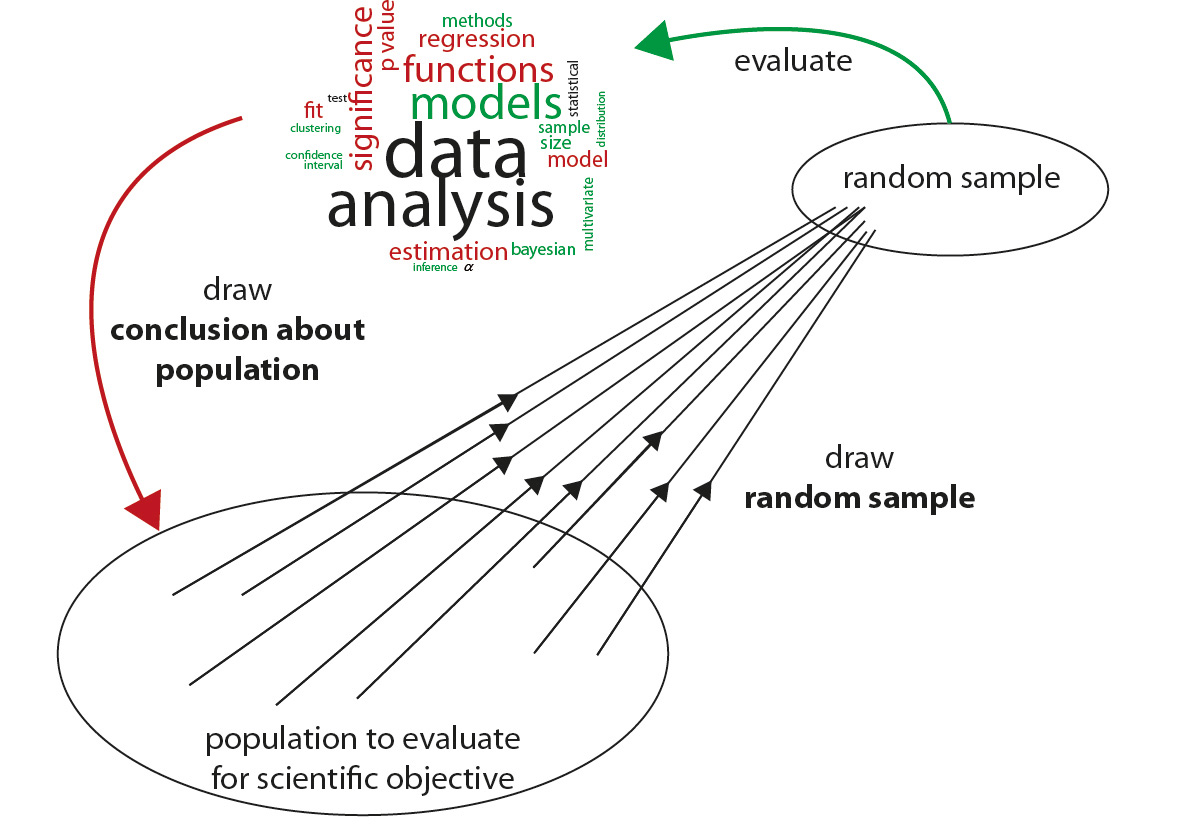
\includegraphics[width=.7\linewidth]{inference.jpg}
  \end{center}
\end{frame}

\begin{frame}{Type-1 Diabetes (T1D) data}
  \begin{itemize}
    \item $9627$ samples from human population
    \item Classified as diabetic or non-diabetic
    \item Genotyped for T1D risk genes
  \end{itemize}
  \tiny
\begin{kframe}
\begin{alltt}
\hlkwd{xtable}\hlstd{(t1d[}\hlkwd{sample}\hlstd{(}\hlkwd{nrow}\hlstd{(t1d))[}\hlnum{1}\hlopt{:}\hlnum{10}\hlstd{],])}
\end{alltt}
\end{kframe}% latex table generated in R 3.1.1 by xtable 1.7-4 package
% Mon Oct 20 09:53:02 2014
\begin{table}[ht]
\centering
\begin{tabular}{rlrlrlrrrrrr}
  \hline
 & t1d & hlacat & sex & age & european & ptpn22 & il10 & ctla4 & bach2 & erbb3 & gab3 \\ 
  \hline
5595 & yes &   3 & f & 8.84 & TRUE &   1 &   1 &   2 &   0 &   1 &   1 \\ 
  682 & yes &   6 & f & 11.13 & TRUE &   1 &   2 &   2 &   1 &   0 &   0 \\ 
  7182 & yes &   2 & m & 4.85 & TRUE &   0 &   2 &   1 &   1 &   1 &   0 \\ 
  9297 & no &   1 & f & 9.80 & TRUE &   0 &   1 &   2 &   2 &   1 &   0 \\ 
  8139 & yes &   1 & f & 8.09 & TRUE &   0 &   2 &   1 &   0 &   2 &   0 \\ 
  7620 & no &   2 & f & 6.44 & TRUE &   0 &   1 &   1 &   1 &   2 &   0 \\ 
  1564 & yes &   6 & m & 11.04 & TRUE &   0 &   2 &   1 &   0 &   1 &   0 \\ 
  1195 & yes &   6 & f & 13.89 & TRUE &   1 &   2 &   2 &   1 &   2 &   1 \\ 
  7361 & yes &   2 & m & 6.02 & TRUE &   1 &   2 &   1 &   0 &   0 &   0 \\ 
  2 & yes &   6 & m & 6.64 & TRUE &   0 &   2 &   1 &   2 &   0 &   0 \\ 
   \hline
\end{tabular}
\end{table}

\end{frame}

\begin{frame}{T1D variables}
  \begin{itemize}
    \item $Y$: \textbf{Output variable}, \textbf{target variable}
      \begin{itemize}
        \item T1D yes or no
      \end{itemize}
    \item $X_i$: \textbf{Input variables}, \textbf{explanatory variables}, 
      \textbf{covariates}
      \begin{itemize}
        \item Sex
        \item Age
        \item European
        \item PTPN22, IL10, CTLA4, ...
      \end{itemize}
  \end{itemize}
\end{frame}

\begin{frame}{Types of variables}
  \begin{columns}[t]
    \begin{column}{.45\linewidth}
      \begin{exampleblock}{Discrete}
        \begin{itemize}
          \item $X \in \{s_1, s_2, \dots, s_n\}$
          \item {\bf Binary} 
            \\ $\text{european} \in \{\text{TRUE}, \text{FALSE}\}$
          \item {\bf Categorical} \\ 
            $\text{sex} \in \{\text{f}, \text{m}\}$
          \item {\bf Ordinal} 
            \\ $\text{age} \in \{\text{child}, \text{adult}, \text{elder}\}$
          \item {\bf Integer} 
            \\ $\text{ptpn22} \in \{0, 1, 2\}$
        \end{itemize}
      \end{exampleblock}
    \end{column}
    \begin{column}{.45\linewidth}
      \begin{exampleblock}{Continuous}
        \begin{itemize}
          \item $X \in \mathbb{R}$
          \item $\text{age} \in [0, 0.01, \dots, \inf[$
        \end{itemize}
      \end{exampleblock}
    \end{column}
  \end{columns}
  \begin{align*}
    \text{Binary} < \text{Categorical} < \text{Ordinal} < \text{Integer} <
    \text{Continuous}
  \end{align*}
\end{frame}

\begin{frame}{Operations on variables}
  \begin{description}
    \item[Count] Binary, categorical, ordinal, integer, continuous
    \item[Median] Ordinal, integer, continuous
    \item[Median] Ordinal, integer, continuous
    \item[Mean] Integer, continuous
  \end{description}
\end{frame}

\begin{frame}[fragile]{Count}
  \begin{definition}[Count]
    \begin{itemize}
      \item How often does $x$ appear?
      \item Binary, categorical, ordinal, integer, continuous
    \end{itemize}
  \end{definition}
\begin{knitrout}\tiny
\definecolor{shadecolor}{rgb}{0.969, 0.969, 0.969}\color{fgcolor}\begin{kframe}
\begin{alltt}
\hlkwd{table}\hlstd{(t1d}\hlopt{$}\hlstd{t1d)}
\end{alltt}
\begin{verbatim}
## 
##   no  yes 
## 1766 7861
\end{verbatim}
\begin{alltt}
\hlkwd{table}\hlstd{(t1d}\hlopt{$}\hlstd{sex)}
\end{alltt}
\begin{verbatim}
## 
##    f    m 
## 4721 4906
\end{verbatim}
\end{kframe}
\end{knitrout}
\end{frame}

\begin{frame}[fragile]{Median}
  \begin{definition}[Median]
    \begin{itemize}
      \item Value in the middle
      \item Ordinal, integer, continuous
    \end{itemize}
  \end{definition}
\begin{knitrout}\tiny
\definecolor{shadecolor}{rgb}{0.969, 0.969, 0.969}\color{fgcolor}\begin{kframe}
\begin{alltt}
\hlkwd{median}\hlstd{(t1d}\hlopt{$}\hlstd{hlacat)}
\end{alltt}
\begin{verbatim}
## [1] 3
\end{verbatim}
\begin{alltt}
\hlkwd{median}\hlstd{(t1d}\hlopt{$}\hlstd{age)}
\end{alltt}
\begin{verbatim}
## [1] 7.99
\end{verbatim}
\end{kframe}
\end{knitrout}
\end{frame}

\begin{frame}[fragile]{Quantile}
  \begin{definition}[Quantile]
    \begin{itemize}
      \item $q_p(X)$ is value $x$, s.t. $q\%$ of all $y \in Y$ are smaller than $x$
      \item $q_{0.5}(X) = \operatorname{median}(X)$
      \item Ordinal, integer, continuous
    \end{itemize}
  \end{definition}
\begin{knitrout}\tiny
\definecolor{shadecolor}{rgb}{0.969, 0.969, 0.969}\color{fgcolor}\begin{kframe}
\begin{alltt}
\hlkwd{quantile}\hlstd{(t1d}\hlopt{$}\hlstd{hlacat)}
\end{alltt}
\begin{verbatim}
##   0%  25%  50%  75% 100% 
##    1    2    3    6    6
\end{verbatim}
\begin{alltt}
\hlkwd{quantile}\hlstd{(t1d}\hlopt{$}\hlstd{age)}
\end{alltt}
\begin{verbatim}
##     0%    25%    50%    75%   100% 
##  0.000  5.234  7.990 10.674 22.138
\end{verbatim}
\end{kframe}
\end{knitrout}
\end{frame}

\begin{frame}[fragile]{Mean}
  \begin{definition}[Mean]
    \begin{itemize}
      \item $\operatorname{mean}(X) = \frac{1}{|X|}\sum_{x \in X} x$
      \item Integer, continuous variables
    \end{itemize}
  \end{definition}
\begin{knitrout}\tiny
\definecolor{shadecolor}{rgb}{0.969, 0.969, 0.969}\color{fgcolor}\begin{kframe}
\begin{alltt}
\hlkwd{mean}\hlstd{(t1d}\hlopt{$}\hlstd{age)}
\end{alltt}
\begin{verbatim}
## [1] 7.976
\end{verbatim}
\end{kframe}
\end{knitrout}
\end{frame}

\begin{frame}{Random variable}
  \begin{itemize}
    \item A random variable $X$ has a random outcome $x \in \mathcal{D}$
    \item $\mathcal{D}$ is the \textbf{domain} of $X$
    \item \textbf{Discrete $X$}: $\mathcal{D} \subseteq \mathbb{Z}$, e.g. $\mathbb{D}=\{0, 1, 2, \dots\}$
    \item \textbf{Continuous $X$}: $\mathcal{D} \subseteq \mathbb{R}$, e.g. $\mathbb{D}=[0.0, 0.1, 0.2, \dots[$
    \item $P(X=x)$ is the \textbf{probability} that $X$ has outcome $x$
    \item $E[X]=\sum_{x \in \mathcal{D}} P(X=x) x$ is the \textbf{expected value} of $X$
    \item $Var[X]=\sum_{x \in \mathcal{D}} P(X=x) (x - E[X])^2$ is the \textbf{variance} of $X$
    \item $Sd[X]=\sqrt{Var[X]}$ is the \textbf{standard deviation} of $X$
  \end{itemize}
\end{frame}

\begin{frame}{Discrete Random Variable}
  \begin{itemize}
    \item $f(x) = P(X=x)$ is the \textbf{Probability Mass Function (PMF)} of $X$
    \item $F(X) = P(X\le x)$ is the \textbf{Cumulative Distribution Function (CDF)} of $X$
  \end{itemize}
  \begin{exampleblock}{Examples}
    \begin{itemize}
      \item $\operatorname{Bernoulli}(p)$: $\mathcal{D} = \{0, 1\}$
      \item $\operatorname{Binomial}(n, p)$: $\mathcal{D} = \{0, 1, \dots, n\}$
      \item $\operatorname{Poisson}(\lambda)$: $\mathcal{D} = \{0, 1, \dots, +\inf\}$
    \end{itemize}
  \end{exampleblock}
\end{frame}

\begin{frame}[fragile]{Bernoulli distribution}
  \begin{itemize}
    \item The gender $X$ with $\mathcal{D}=\{f, m\}$ can be modelled as
      Bernoulli distributed:
  \end{itemize}
  \begin{columns}
    \begin{column}{.5\linewidth}
      \begin{align*}
        X \sim \operatorname{Bernoulli}(p)
      \end{align*}
      \begin{align*}
        E[X] = p
      \end{align*}
      \begin{align*}
        Var[X] = p(1-p)
      \end{align*}
    \end{column}
    \begin{column}{0.5\linewidth}
\begin{knitrout}\tiny
\definecolor{shadecolor}{rgb}{0.969, 0.969, 0.969}\color{fgcolor}\begin{kframe}
\begin{alltt}
\hlstd{p} \hlkwb{<-} \hlnum{0.65}
\hlstd{exp} \hlkwb{<-} \hlstd{p}
\hlstd{samples} \hlkwb{<-} \hlkwd{rbinom}\hlstd{(}\hlnum{100}\hlstd{,} \hlnum{1}\hlstd{, p)}
\hlkwd{hist}\hlstd{(samples,} \hlkwc{col}\hlstd{=}\hlstr{'lightblue'}\hlstd{,} \hlkwc{main}\hlstd{=}\hlstr{''}\hlstd{,} \hlkwc{xlab}\hlstd{=}\hlstr{''}\hlstd{)}
\hlkwd{abline}\hlstd{(}\hlkwc{v}\hlstd{=exp,} \hlkwc{col}\hlstd{=}\hlstr{'red'}\hlstd{,} \hlkwc{lwd}\hlstd{=}\hlnum{2}\hlstd{)}
\end{alltt}
\end{kframe}

{\centering \includegraphics[width=\linewidth]{figure/hist_bernoulli} 

}



\end{knitrout}
    \end{column}
  \end{columns}
\end{frame}

\begin{frame}[fragile]{Bernoulli distribution}
  \begin{itemize}
    \item What is the rate $p$ of females?
    \item The \textbf{maximum likelihood} estimator $\hat{p}$ of $p$ is:
      \begin{align*}
        \hat{p}=\frac{1}{n}\sum_i x_i
      \end{align*}
\begin{knitrout}\tiny
\definecolor{shadecolor}{rgb}{0.969, 0.969, 0.969}\color{fgcolor}\begin{kframe}
\begin{alltt}
\hlstd{p} \hlkwb{<-} \hlkwd{sum}\hlstd{(t1d}\hlopt{$}\hlstd{sex} \hlopt{==} \hlstr{'f'}\hlstd{)} \hlopt{/} \hlkwd{nrow}\hlstd{(t1d)}
\hlstd{p}
\end{alltt}
\begin{verbatim}
## [1] 0.4904
\end{verbatim}
\end{kframe}
\end{knitrout}
  \end{itemize}
\end{frame}

\begin{frame}[fragile]{Binomial distribution}
  \begin{itemize}
    \item The number of females $Y$ in a new cohort of $n=50$ people is
      binomial distributed:
      \begin{align*}
        Y \sim \operatorname{Binomial}(n, p)
      \end{align*}
    \item Assume that $p=\hat{p}=0.4904$ is the same as before ...
  \end{itemize}
\end{frame}

\begin{frame}[fragile]{Binomial distribution}
  \begin{itemize}
    \item then the probability $f(y)$ to observe $k$ females is:
  \end{itemize}
\begin{knitrout}\tiny
\definecolor{shadecolor}{rgb}{0.969, 0.969, 0.969}\color{fgcolor}\begin{kframe}
\begin{alltt}
\hlstd{n} \hlkwb{<-} \hlnum{50}
\hlstd{y} \hlkwb{<-} \hlkwd{seq}\hlstd{(}\hlnum{0}\hlstd{, n)}
\hlstd{f_y} \hlkwb{<-} \hlkwd{dbinom}\hlstd{(y, n, p)}
\hlstd{d} \hlkwb{<-} \hlkwd{data.frame}\hlstd{(}\hlkwc{x}\hlstd{=y,} \hlkwc{y}\hlstd{=f_y)}
\hlkwd{ggplot}\hlstd{(d,} \hlkwd{aes}\hlstd{(}\hlkwc{x}\hlstd{=x,} \hlkwc{y}\hlstd{=y))} \hlopt{+} \hlkwd{geom_point}\hlstd{(}\hlkwc{color}\hlstd{=}\hlstr{'blue'}\hlstd{,} \hlkwc{size}\hlstd{=}\hlnum{3}\hlstd{)} \hlopt{+} \hlkwd{xlab}\hlstd{(}\hlstr{'y'}\hlstd{)} \hlopt{+} \hlkwd{ylab}\hlstd{(}\hlstr{'f(y)'}\hlstd{)}
\end{alltt}
\end{kframe}

{\centering \includegraphics[width=.5\linewidth]{figure/fig_bin_pdf} 

}



\end{knitrout}
\end{frame}

\begin{frame}[fragile]{Binomial distribution}
  \begin{itemize}
    \item and the probability $F(Y)$ to observe up to $k$ females:
  \end{itemize}
\begin{knitrout}\tiny
\definecolor{shadecolor}{rgb}{0.969, 0.969, 0.969}\color{fgcolor}\begin{kframe}
\begin{alltt}
\hlstd{n} \hlkwb{<-} \hlnum{50}
\hlstd{y} \hlkwb{<-} \hlkwd{seq}\hlstd{(}\hlnum{0}\hlstd{, n)}
\hlstd{F_y} \hlkwb{<-} \hlkwd{pbinom}\hlstd{(y, n, p)}
\hlstd{d} \hlkwb{<-} \hlkwd{data.frame}\hlstd{(}\hlkwc{x}\hlstd{=y,} \hlkwc{y}\hlstd{=F_y)}
\hlkwd{ggplot}\hlstd{(d,} \hlkwd{aes}\hlstd{(}\hlkwc{x}\hlstd{=x,} \hlkwc{y}\hlstd{=y))} \hlopt{+} \hlkwd{geom_point}\hlstd{(}\hlkwc{color}\hlstd{=}\hlstr{'blue'}\hlstd{,} \hlkwc{size}\hlstd{=}\hlnum{3}\hlstd{)} \hlopt{+} \hlkwd{xlab}\hlstd{(}\hlstr{'y'}\hlstd{)} \hlopt{+} \hlkwd{ylab}\hlstd{(}\hlstr{'F(y)'}\hlstd{)}
\end{alltt}
\end{kframe}

{\centering \includegraphics[width=.5\linewidth]{figure/fig_bin_cdf} 

}



\end{knitrout}
\end{frame}

\begin{frame}{Continuous Random Variable}
  \begin{itemize}
    \item $f(x) = P(X \in ]x-\epsilon;x+\epsilon[)$ is the \textbf{Probability Density Function (PDF)} of $X$
    \item $F(X) = P(X\le x)$ is the \textbf{Cumulative Distribution Function (CDF)} of $X$
  \end{itemize}
  \begin{exampleblock}{Examples}
    \begin{itemize}
      \item $\operatorname{Normal}(\mu, \sigma^2)$: $\mathcal{D} = \mathbb{R}$ 
      \item $\operatorname{Exponential}(\lambda)$: $\mathcal{D} = \mathbb{R}^+$
      \item $\operatorname{Beta}(a, b)$: $\mathcal{D} = [0, \dots, 1]$
    \end{itemize}
  \end{exampleblock}
\end{frame}

\begin{frame}[fragile]{Normal distribution}
  \begin{itemize}
    \item $X \sim N(\mu, \sigma^2)$
    \item $E[X]=\mu$, $Var[X]=\sigma^2$
    \item $Z \sim N(0, 1)$ is \textbf{standard normal} distribution
    \item $X \sim N(\mu, \sigma^2) \rightarrow \frac{X-\mu}{\sigma} \sim N(0,1)$
  \end{itemize}
\begin{knitrout}\tiny
\definecolor{shadecolor}{rgb}{0.969, 0.969, 0.969}\color{fgcolor}\begin{kframe}
\begin{alltt}
\hlstd{x} \hlkwb{<-} \hlkwd{seq}\hlstd{(}\hlopt{-}\hlnum{10}\hlstd{,} \hlnum{10}\hlstd{,} \hlkwc{len}\hlstd{=}\hlnum{100}\hlstd{)}
\hlstd{y} \hlkwb{<-} \hlkwd{dnorm}\hlstd{(x,} \hlkwc{mean}\hlstd{=}\hlnum{0}\hlstd{,} \hlkwc{sd}\hlstd{=}\hlnum{1.0}\hlstd{)}
\hlstd{d} \hlkwb{<-} \hlkwd{data.frame}\hlstd{(}\hlkwc{x}\hlstd{=x,} \hlkwc{y}\hlstd{=y)}
\hlkwd{ggplot}\hlstd{(d,} \hlkwd{aes}\hlstd{(}\hlkwc{x}\hlstd{=x,} \hlkwc{y}\hlstd{=y))} \hlopt{+} \hlkwd{geom_line}\hlstd{(}\hlkwc{color}\hlstd{=}\hlstr{'blue'}\hlstd{,} \hlkwc{size}\hlstd{=}\hlnum{2}\hlstd{)} \hlopt{+} \hlkwd{xlab}\hlstd{(}\hlstr{'x'}\hlstd{)} \hlopt{+} \hlkwd{ylab}\hlstd{(}\hlstr{'f(x)'}\hlstd{)}
\end{alltt}
\end{kframe}

{\centering \includegraphics[width=.6\linewidth]{figure/normal} 

}



\end{knitrout}
\end{frame}

\begin{frame}[fragile]{Example}
  \begin{itemize}
    \item How is the \textbf{age} distributed in the T1D cohort?
  \end{itemize}
\begin{knitrout}\tiny
\definecolor{shadecolor}{rgb}{0.969, 0.969, 0.969}\color{fgcolor}\begin{kframe}
\begin{alltt}
\hlkwd{hist}\hlstd{(t1d}\hlopt{$}\hlstd{age,} \hlkwc{col}\hlstd{=}\hlstr{'grey'}\hlstd{,} \hlkwc{xlab}\hlstd{=}\hlstr{'Age'}\hlstd{,} \hlkwc{ylab}\hlstd{=}\hlstr{'Density'}\hlstd{,} \hlkwc{prob}\hlstd{=}\hlnum{TRUE}\hlstd{,} \hlkwc{main}\hlstd{=}\hlkwa{NULL}\hlstd{,} \hlkwc{ylim}\hlstd{=}\hlkwd{c}\hlstd{(}\hlnum{0}\hlstd{,} \hlnum{0.12}\hlstd{))}
\end{alltt}
\end{kframe}

{\centering \includegraphics[width=.8\linewidth]{figure/hist_age} 

}



\end{knitrout}
\end{frame}

\begin{frame}[fragile]{Example}
  \begin{itemize}
    \item Estimate $\mu$ and $\sigma$ via maximum likelihood:
  \end{itemize}
\begin{knitrout}\tiny
\definecolor{shadecolor}{rgb}{0.969, 0.969, 0.969}\color{fgcolor}\begin{kframe}
\begin{alltt}
\hlstd{mu} \hlkwb{<-} \hlkwd{mean}\hlstd{(t1d}\hlopt{$}\hlstd{age)}
\hlstd{sigma} \hlkwb{<-} \hlkwd{sd}\hlstd{(t1d}\hlopt{$}\hlstd{age)}
\hlstd{x} \hlkwb{<-} \hlkwd{seq}\hlstd{(}\hlkwd{min}\hlstd{(t1d}\hlopt{$}\hlstd{age),} \hlkwd{max}\hlstd{(t1d}\hlopt{$}\hlstd{age),} \hlkwc{len}\hlstd{=}\hlnum{100}\hlstd{)}
\hlstd{y} \hlkwb{<-} \hlkwd{dnorm}\hlstd{(x,} \hlkwc{mean}\hlstd{=mu,} \hlkwc{sd}\hlstd{=sigma)}
\hlkwd{hist}\hlstd{(t1d}\hlopt{$}\hlstd{age,} \hlkwc{col}\hlstd{=}\hlstr{'grey'}\hlstd{,} \hlkwc{xlab}\hlstd{=}\hlstr{'Age'}\hlstd{,} \hlkwc{ylab}\hlstd{=}\hlstr{'Density'}\hlstd{,} \hlkwc{prob}\hlstd{=}\hlnum{TRUE}\hlstd{,} \hlkwc{main}\hlstd{=}\hlkwa{NULL}\hlstd{,} \hlkwc{ylim}\hlstd{=}\hlkwd{c}\hlstd{(}\hlnum{0}\hlstd{,} \hlnum{0.12}\hlstd{))}
\hlkwd{lines}\hlstd{(x, y,} \hlkwc{col}\hlstd{=}\hlstr{'blue'}\hlstd{,} \hlkwc{lwd}\hlstd{=}\hlnum{3}\hlstd{)}
\end{alltt}
\end{kframe}

{\centering \includegraphics[width=.8\linewidth]{figure/hist_normal__k-age} 

}



\end{knitrout}
\end{frame}
 
%knit_child('ht/main.Rnw')
%knit_child('pca/main.Rnw')
%knit_child('clust/main.Rnw')

\end{document}
